\chapter{Algorytm animacji awatara}
\label{cha:implementacja}
Jak wspomniano we wcześniejszych rozdziałach, działanie algorytmu zaimplementowanego na potrzeby tej pracy inżynierskiej można podzielić na kilka kluczowych etapów. Poniższy rozdział zawiera szczegółowy opis każdego z nich. Zostaną także zaprezentowane efekty otrzymane w konkretnych krokach.

% %---------------------------------------------------------------------------

\section{Struktura programu}
Do stworzenia algorytmu wykorzystano język programowania Python umożliwiający tworzenie aplikacji, których działanie oparte jest na wykorzystaniu różnego rodzaju napisanych wcześniej funkcji. W przypadku owego projektu zostały one zaimplementowane dla każdego istotnego etapu programu, które przedstawiono na Rys. \ref{fig:algorithmStructure}.

\begin{figure}[h]
	\centering
	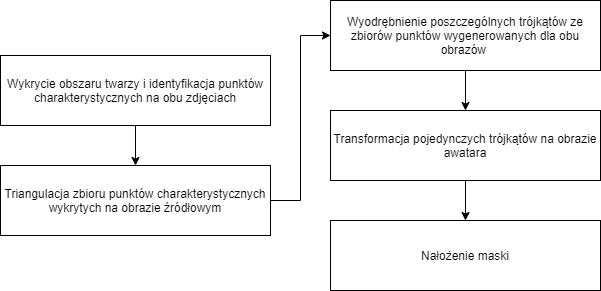
\includegraphics[width=14cm]{zdjęcia/structure.png}
	\caption{Etapy algorytmu animacji awatara} 
	\label{fig:algorithmStructure}
\end{figure}

Kluczową kwestią jest wcześniejsze wczytanie danych, czyli obrazu źródłowego, przez który rozumie się zdjęcie mające posłużyć jako baza do przekształcenia awatara oraz jego obraz, na którym nastąpi animacja. Funkcja łącząca wszystkie działania została przedstawiona w formie poniższego kodu. Jej wynikiem jest obraz awatara ze zmienionym wyrazem twarzy osiągniętym za pomocą odpowiednich przekształceń. W dalszych sekcjach, zostaną opisane poszczególne moduły, z których korzystano.

\begin{minted}
[
frame=lines,
label=Główna funkcja algorytmu,
framesep=2mm,
baselinestretch=1.2,
breaklines,
bgcolor=white,
fontsize=\footnotesize,
linenos
]
{python}
def animate_avatar(avatar_img, avatar_points, src_img, src_points):
    new_avatar_face = np.zeros(src_img.shape, np.uint8)

    for src_triangle_points, avatar_triangle_points in delaunay_triangulation(src_points, avatar_points):
        avatar_img_cropped, avatar_triangle, _ = crop_single_triangle(avatar_triangle_points, avatar_img)
        src_img_cropped, src_triangle, b_rect = crop_single_triangle(src_triangle_points, src_img)

        warped_triangle = transform_triangle(avatar_triangle, avatar_img_cropped, src_triangle, src_img_cropped)
        add_triangle_to_new_face_area(new_avatar_face, warped_triangle, b_rect)

    return generate_new_face(avatar_img, avatar_points, new_avatar_face, src_points)
\end{minted}

% %---------------------------------------------------------------------------

\section{Wykrycie twarzy oraz punktów charakterystynczych}
Pierwszym krokiem jest wykrycie obszaru twarzy oraz identyfikacja jej punktów charakterystycznych. Etap ten został zrealizowany z użyciem gotowych funkcji udostępnianych przez bibliotekę dlib:
\begin{itemize}
    \item \textit{get\_frontal\_face\_detector()} - funkcja nie przyjmuje żadnych parametrów, zwraca wytrenowany obiekt umożliwiający detekcję twarzy. Model został wyszkolony przy pomocy algorytmu działającego w oparciu o klasyfikator SVM i deskryptor HOG, opisany w podrozdziale \ref{sec:svmhog}. 
    \item \textit{shape\_predictor()} - parametrem wejściowym jest wytrenowany model, który również został udostępniony przez bibliotekę, umożliwiający poprawną lokalizację punktów charakterystycznych \cite{dlibModel}. Został on wyszkolony na podstawie algorytmu przedstawionego w sekcji~\ref{sec:landmarks}. Wynikiem zastosowania danej funkcji jest obiekt, który generuje owy zestaw punktów zlokalizowanych na obrazie przekazanym jako dane wejściowe.
\end{itemize}

\begin{minted}
[
frame=lines,
label=Wykrycie twarzy oraz punktów charakterystycznych,
framesep=2mm,
baselinestretch=1.2,
breaklines,
bgcolor=white,
fontsize=\footnotesize,
linenos
]
{python}
def detect_face_and_landmarks(img):
    detector = dlib.get_frontal_face_detector()
    predictor = dlib.shape_predictor('./data/shape_predictor_68_face_landmarks.dat')

    gray = cv2.cvtColor(imutils.resize(img), cv2.COLOR_BGR2GRAY)
    rects = detector(gray, 1)
    facial_landmarks = []

    if rects:
        for rect in rects:
            facial_landmarks = predictor(gray, rect)
            facial_landmarks = face_utils.shape_to_np(facial_landmarks)

    return img, facial_landmarks
\end{minted}

Wybrane funkcje zdają się być wystarczające do osiągnięcia zamierzonego rezultatu. Można założyć, iż przetwarzane obrazy zawierają dobrze widoczny obszar twarzy ustawionej w pozycji frontowej. Z tego powodu dokładność działania narzędzia wykrywającego twarz oraz punkty charakterystyczne jest wysoka.

\begin{figure}[h]
	\centering
	\begin{subfigure}{0.35\textwidth}
		\centering
		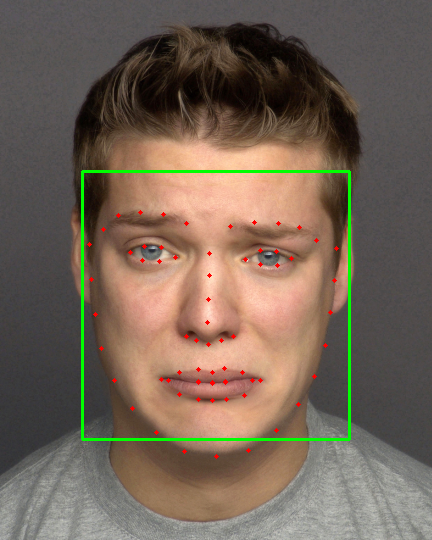
\includegraphics[height=5.5cm]{zdjęcia/detected_landmarks_src.png}
		\subcaption{\label{detected_landmarks_src}}
	\end{subfigure}
	\begin{subfigure}{0.35\textwidth}
		\centering
		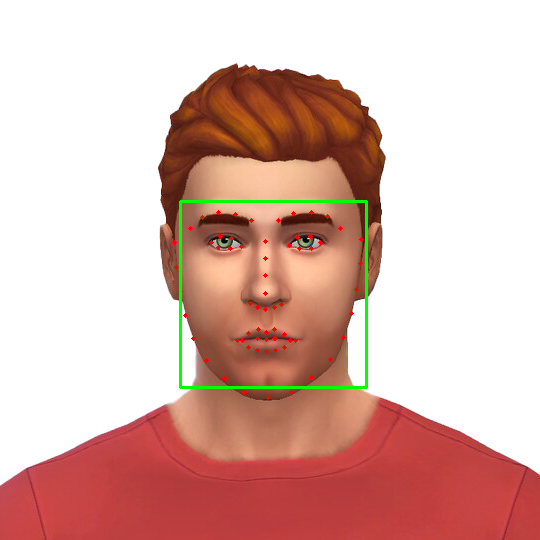
\includegraphics[height=5.5cm]{zdjęcia/detected_landmarks_avatar.png}
		\subcaption{\label{detected_landmarks_avatar}}
	\end{subfigure}
	
	\caption{\label{fig:detectedLandmarks}Elementy wykryte na obrazie źródłowym \protect\subref{detected_landmarks_src} \cite{data} oraz na awatarze \protect\subref{detected_landmarks_avatar} \cite{avatars}}
\end{figure}

Efektem wizualnym użycia powyższej funkcji są obrazy przedstawione na Rys.\ref{fig:detectedLandmarks}. Na każdym ze zdjęć została zlokalizowana twarz, którą zaznaczono zielonym prostokątem oraz jej kluczowe elementy, w postaci 68 punktów oznaczonych kolorem czerwonym. W następnych etapach posłużą one jako baza, na której będą wykonywane wszelkie operacje. 

% \inputminted[firstline=2, lastline=12]{octave}{BitXorMatrix.m}

% %---------------------------------------------------------------------------

\section{Triangulacja zbioru punktów}
Kolejnym etapem algorytmu animacji awatara jest triangulacja zbioru punktów charakterystycznych, zlokalizowanych na obszarze twarzy obrazu źródłowego. Celem jej zastosowania jest podział przestrzeni na nieskomplikowane trójkąty posiadające ostre kąty, co zapewni przejrzystość i równomierność figur.

W bibliotece OpenCV dostępne są funkcje, generujące triangulację Delone dla zestawu punktów. Ich użycie jest bardzo proste i intuicyjne. Z wykorzystaniem modułu \textit{Subdiv2D( Rect rect )}, dla którego parametrem wejściowym jest prostokątny obszar obejmujący wszystkie istotne punkty, zostaje wygenerowany pusty obiekt. Następnie za pomocą funkcji \textit{insert()} można dodać do niego elementy charakterystyczne, dla których chcemy dokonać triangulacji. Ostatnim krokiem jest wywołanie funkcji \textit{getTriangleList()}, która zwraca listę trójkątów wygenerowanych przez algorytm. 

\begin{minted}
[
frame=lines,
label=Triangulacja Delone dla zbioru punktów,
framesep=2mm,
baselinestretch=1.2,
breaklines,
bgcolor=white,
fontsize=\footnotesize,
linenos
]
{python}
def delaunay_triangulation(src_points, avatar_points):
    points_list = list(src_points)
    delaunay_subdivision = cv2.Subdiv2D((*src_points.min(axis=0), *src_points.max(axis=0)))
    delaunay_subdivision.insert(points_list)

    for x1, y1, x2, y2, x3, y3 in delaunay_subdivision.getTriangleList():
        indexes_set = [(src_points == single_point).all(axis=1).nonzero()[0][0]
                       for single_point in [[x1, y1], [x2, y2], [x3, y3]]]

        src_triangles = generate_xy_for_indexes(src_points, indexes_set)
        avatar_triangles = generate_xy_for_indexes(avatar_points, indexes_set)
        yield [np.array(src_triangles), np.array(avatar_triangles)]
        

def generate_xy_for_indexes(points, indexes):
    return [points[single_index] for single_index in indexes]
\end{minted}

Funkcja zaimplementowana w celu rozwiązania tej części problemu generuje opisaną powyżej triangulację. Kolejną istotną kwestią jest wyodrębnienie analogicznych trójkątów z obydwu zbiorów punktów. Moduł \textit{getTriangleList()} zwraca współrzędne wszystkich trzech wierzchołków każdego z wygenerowanych trójkątów. W prosty sposób można odnaleźć ich indeksy w~zbiorze punktów charakterystycznych obrazu źródłowego, a następnie zidentyfikować analogiczne elementy w~zbiorze punktów wygenerowanych z obrazu awatara.

\begin{figure}[h]
	\centering
	\begin{subfigure}{0.35\textwidth}
		\centering
		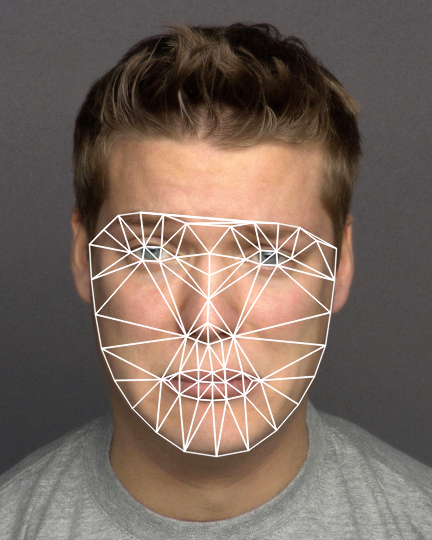
\includegraphics[height=5.5cm]{zdjęcia/triangulation_src.png}
		\subcaption{\label{triangulation_src}}
	\end{subfigure}
	\begin{subfigure}{0.35\textwidth}
		\centering
		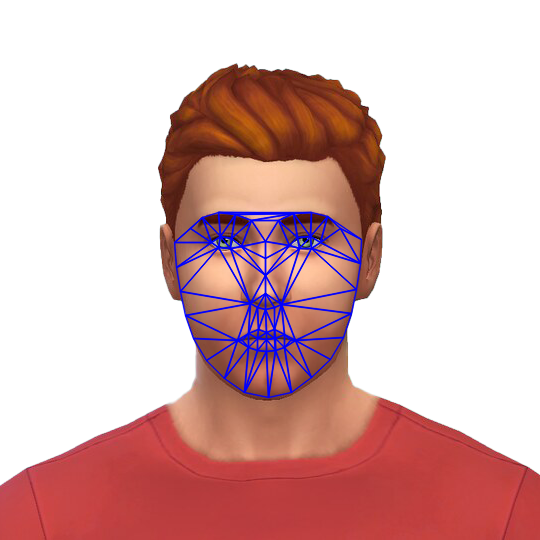
\includegraphics[height=5.5cm]{zdjęcia/triangulation_avatar.png}
		\subcaption{\label{triangulation_avatar}}
	\end{subfigure}
	
	\caption{\label{fig:triangulation}Triangulacja punktów char. obrazu źródłowego \protect\subref{triangulation_src} oraz awatara \protect\subref{triangulation_avatar}}
\end{figure}

Na Rys. \ref{fig:triangulation} można zaobserwować efekt działania tego etapu programu. Na pierwszym obrazie zaznaczono trójkąty otrzymane w wyniku zastosowania triangulacji Delone, natomiast na drugim zaznaczono analogicznie wykryte trójkąty. Figury, które zostały otrzymane poprzez użycie funkcji z biblioteki OpenCV umożliwią klarowne wykonanie dalszych transformacji.

% %---------------------------------------------------------------------------

\section{Transformacja trójkątów}
\label{sec:transformacjaTrojkatow}
Posiadając zbiory trójkątów dla obydwu obrazów, można przejść do następnego kroku algorytmu. Jego celem jest dopasowanie każdej z pojedynczych figur obrazu awatara do odpowiadającego mu trójkąta (punkty o tych samych indeksach) z obrazu źródłowego. Mówiąc prościej, należy dokonać transformacji płaszczyzny do odpowiadającego mu obszaru trójkąta.

W celu uzyskania owych rezultatów potrzebna jest funkcja pomocnicza, która przygotuje przetwarzane obszary, tak aby można było dokonać transformacji. Na początku należy wyodrębnić obydwa fragmenty obrazów, w których znajdą się analizowane aktualnie figury. Fragemnt kodu przedstawionego poniżej umożliwia dokonanie tej operacji. Funkcja zwróci przycięty region  oraz nowe współrzędne trójkątów odnoszące się do mniejszego obszaru, a nie całego obrazu. Na Rys. \ref{triangle_src},  \ref{triangle_avatar} przedstawiono efekt zastosowania danego modułu.

\begin{minted}
[
frame=lines,
label=Funkcja pomocnicza przygotowująca trójkąty,
framesep=2mm,
baselinestretch=1.2,
breaklines,
bgcolor=white,
fontsize=\footnotesize,
linenos
]
{python}
def crop_single_triangle(single_triangle, img):
    b_rect = cv2.boundingRect(single_triangle)
    triangle_img = [(indexes[0] - b_rect[0], indexes[1] - b_rect[1]) for indexes in single_triangle]
    cropped_img = img[b_rect[1]:b_rect[1] + b_rect[3], b_rect[0]:b_rect[0] + b_rect[2]]

    return cropped_img, triangle_img, b_rect
\end{minted}



\begin{figure}[h]
	\centering
	\begin{subfigure}{0.35\textwidth}
		\centering
		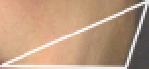
\includegraphics[height=2.5cm]{zdjęcia/triangle_src.png}
		\subcaption{\label{triangle_src}}
	\end{subfigure}
	\begin{subfigure}{0.35\textwidth}
		\centering
		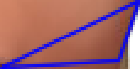
\includegraphics[height=2.5cm]{zdjęcia/triangle_avatar.png}
		\subcaption{\label{triangle_avatar}}
	\end{subfigure}
	\begin{subfigure}{0.35\textwidth}
		\centering
		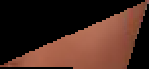
\includegraphics[height=2.5cm]{zdjęcia/triangle_result.png}
		\subcaption{\label{triangle_result}}
	\end{subfigure}

	\caption{\label{fig:triangles}Odpowiadające sobie figury wyodrębnione z obszaru obrazu źródłowego \protect\subref{triangle_src} i awatara \protect\subref{triangle_avatar} oraz rezultat transformacji \protect\subref{triangle_result} płaszczyzny \protect\subref{triangle_avatar} w \protect\subref{triangle_src}}
\end{figure}

Po pobraniu odpowiednich danych dla dwóch przetwarzanych figur, możliwe jest wywołanie kolejnej funkcji, której celem jest transformacja fragmentu obrazu awatara. Skorzystano tutaj z modułów udostępnianych przez bibliotekę OpenCV:

\begin{itemize}
    \item \textit{getAffineTransform()} - jako dane wejściowe należy podać dwa zbiory punktów, dla których obliczana jest macierz transformacji afinicznej.
    \item \textit{warpAffine()} - funkcja dokonuje przekształcenia obrazu za pomocą macierzy rotacji będącej wynikiem wcześniejszej operacji.
\end{itemize}
\begin{minted}
[
frame=lines,
label=Funkcja pomocnicza transformująca trójkąty,
framesep=2mm,
baselinestretch=1.2,
breaklines,
bgcolor=white,
fontsize=\footnotesize,
linenos
]
{python}
def transform_triangle(avatar_triangle, avatar_img_cropped, src_triangle, src_img_cropped):
    transform_matrix = cv2.getAffineTransform(np.float32(avatar_triangle), np.float32(src_triangle))
    warped_triangle = cv2.warpAffine(avatar_img_cropped, transform_matrix,
                                     (src_img_cropped.shape[1], src_img_cropped.shape[0]), None,
                                     flags=cv2.INTER_LINEAR, borderMode=cv2.BORDER_REFLECT_101)

    mask = np.zeros(src_img_cropped.shape, dtype=np.uint8)
    mask = cv2.fillConvexPoly(mask, np.int32(src_triangle), (1.0, 1.0, 1.0), 16, 0)
    
    return warped_triangle *= mask
\end{minted}


Jako wynik otrzymano zmodyfikowany obraz. Na Rys. \ref{triangle_result} zwizualizowano ten krok dla wybranej iteracji. Po otrzymaniu nowej figury, należy dodać ją do obszaru twarzy, który docelowo zastąpi aktualny rejon oblicza awatara. Funkcja \textit{add\_triangle\_to\_new\_rect\_area()} odpowiada za to zadanie. W celu usunięcia ewentualnych szumów etap ten poprzedzono zastosowaniem binaryzacji progowej.



Schemat opisany w tej sekcji należy powtórzyć dla każdego trójkąta zwróconego przez funkcję \textit{delaunay\_triangulation()}. W skończonej pętli następuje modyfikacja wszystkich figur i jednoczesna rekonstrukcja danych fragmentów obszaru twarzy awatara. Finalny efekt można obserwować na Rys. \ref{mask_before_avatar} przedstawionym w następnej sekcji. Trójkąty zostały dopasowane do odpowiadających im figur z obrazu źródłowego, efektem jest zmodyfikowany obszar twarzy o~takich samych wymiarach jak twarz źródłowa (\ref{src_img}).



\begin{minted}
[
frame=lines,
label=Funkcja dodająca transformowaną figurę do nowego obszaru twarzy,
framesep=2mm,
baselinestretch=1.2,
breaklines,
bgcolor=white,
fontsize=\footnotesize,
linenos
]
{python}
def add_triangle_to_new_face_area(new_face, warped_triangle, b_rect):
    (x, y, w, h) = b_rect
    new_face_gray = cv2.cvtColor(new_face[y: y + h, x: x + w], cv2.COLOR_BGR2GRAY)
    _, mask = cv2.threshold(new_face_gray, 0, 255, cv2.THRESH_BINARY_INV)
    warped_triangle = cv2.bitwise_and(warped_triangle, warped_triangle, mask=mask)

    new_face[y: y + h, x: x + w] += warped_triangle
\end{minted}

% %---------------------------------------------------------------------------

\newpage
\section{Nałożenie maski}
Finalnym etapem opisywanego algorytmu jest ponowna transformacja, tym razem całego obszaru nowej twarzy awatara, tak aby odpowiadała ona jej wcześniejszym proporcjom. Ze względu na to, iż funkcja wykorzystana w poprzednim rozdziale (\textit{getAffineTransform()}), przyjmuje pary tylko trzech lub czterech punktów, w tym przypadku użyto innych modułów. Zostały one udostępnione przez bibliotekę scikit-image:

\begin{figure}[h]
	\centering
	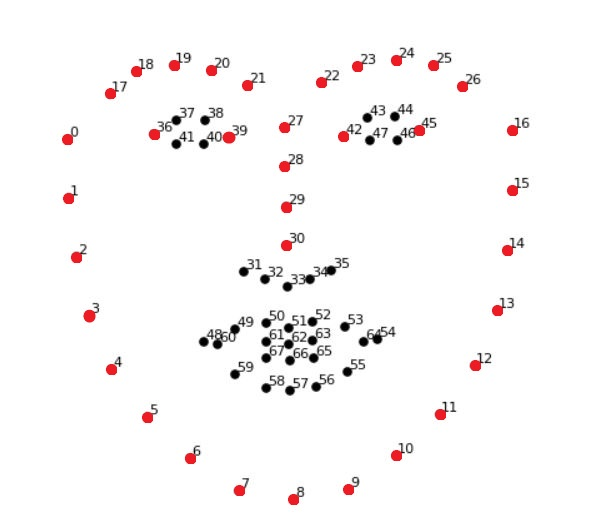
\includegraphics[width=7cm]{zdjęcia/specific_landmarks.JPG}
	\caption{Punkty, na podstawie których następuje ostateczna transformacja} 
	\label{fig:specificLandmarks}
\end{figure}

\begin{itemize}
    \item \textit{PiecewiseAffineTransform()} - inicjalizacja pustego obiektu, który umożliwia transformację bazując na dwóch równoliczncych zestawach punktów. Jej działanie oparte jest na wykorzystaniu triangulacji Delone.
    \item \textit{estimate()} - funkcja wywołana na otrzymanym wcześniej obiekcie przyjmuje dwa zestawy punktów, dla których ma nastapiąć przemapowanie. W przypadku działania owego programu wybrano elementy oznaczone na Rys. \ref{fig:specificLandmarks} kolorem czerwonym. Są to punkty charakterystyczne, które z reguły, w przypadku podstawowych zmian mimiki twarzy pozostają niezmienne - linia szczęki, główny zarys nosa oraz kąciki oczu. Wybór akurat tych punktów zapewni zachowanie odpowiednich proporcji twarzy w trakcie transformacji obszaru.
    \item \textit{warp()} - funkcja dokonująca transformacji płaszczyzny przekazanej jako dane wejściowe.
\end{itemize}

\begin{minted}
[
frame=lines,
framesep=2mm,
baselinestretch=1.2,
breaklines,
bgcolor=white,
fontsize=\footnotesize,
linenos
]
{python}
def generate_new_face(avatar_img, avatar_points, new_avatar_face, src_points):
    transform = PiecewiseAffineTransform()
    transform.estimate(choose_specific_points(avatar_points), choose_specific_points(src_points))

    face = warp(new_avatar_face, transform, output_shape=avatar_img.shape, order=0, mode='wrap')
    face = cv2.normalize(face, None, 0, 255, cv2.NORM_MINMAX, cv2.CV_8U)

    face_gray = cv2.cvtColor(face, cv2.COLOR_BGR2GRAY)
    _, mask = cv2.threshold(face_gray, 0, 255, cv2.THRESH_BINARY_INV)
    new_avatar_img = cv2.bitwise_and(avatar_img, avatar_img, mask=mask)

    new_avatar_img += face

    return new_avatar_img
\end{minted}

Po wykonaniu opisanych instrukcji należy dokonać normalizacji całego obrazu, aby przywrócić odpowiedni typ danych. Na Rys. \ref{mask_after_avatar} przedstawiono rezultat twarzy zmodyfikowanej do odpowiednich wymiarów. Jak widać otrzymany obraz składa się tylko ze zmodyfikowanego obszaru, przez co można swobodnie przejść do próby podmiany danego regionu na obrazie początkowym.

\begin{figure}[h]
	\centering
	\begin{subfigure}{0.35\textwidth}
		\centering
		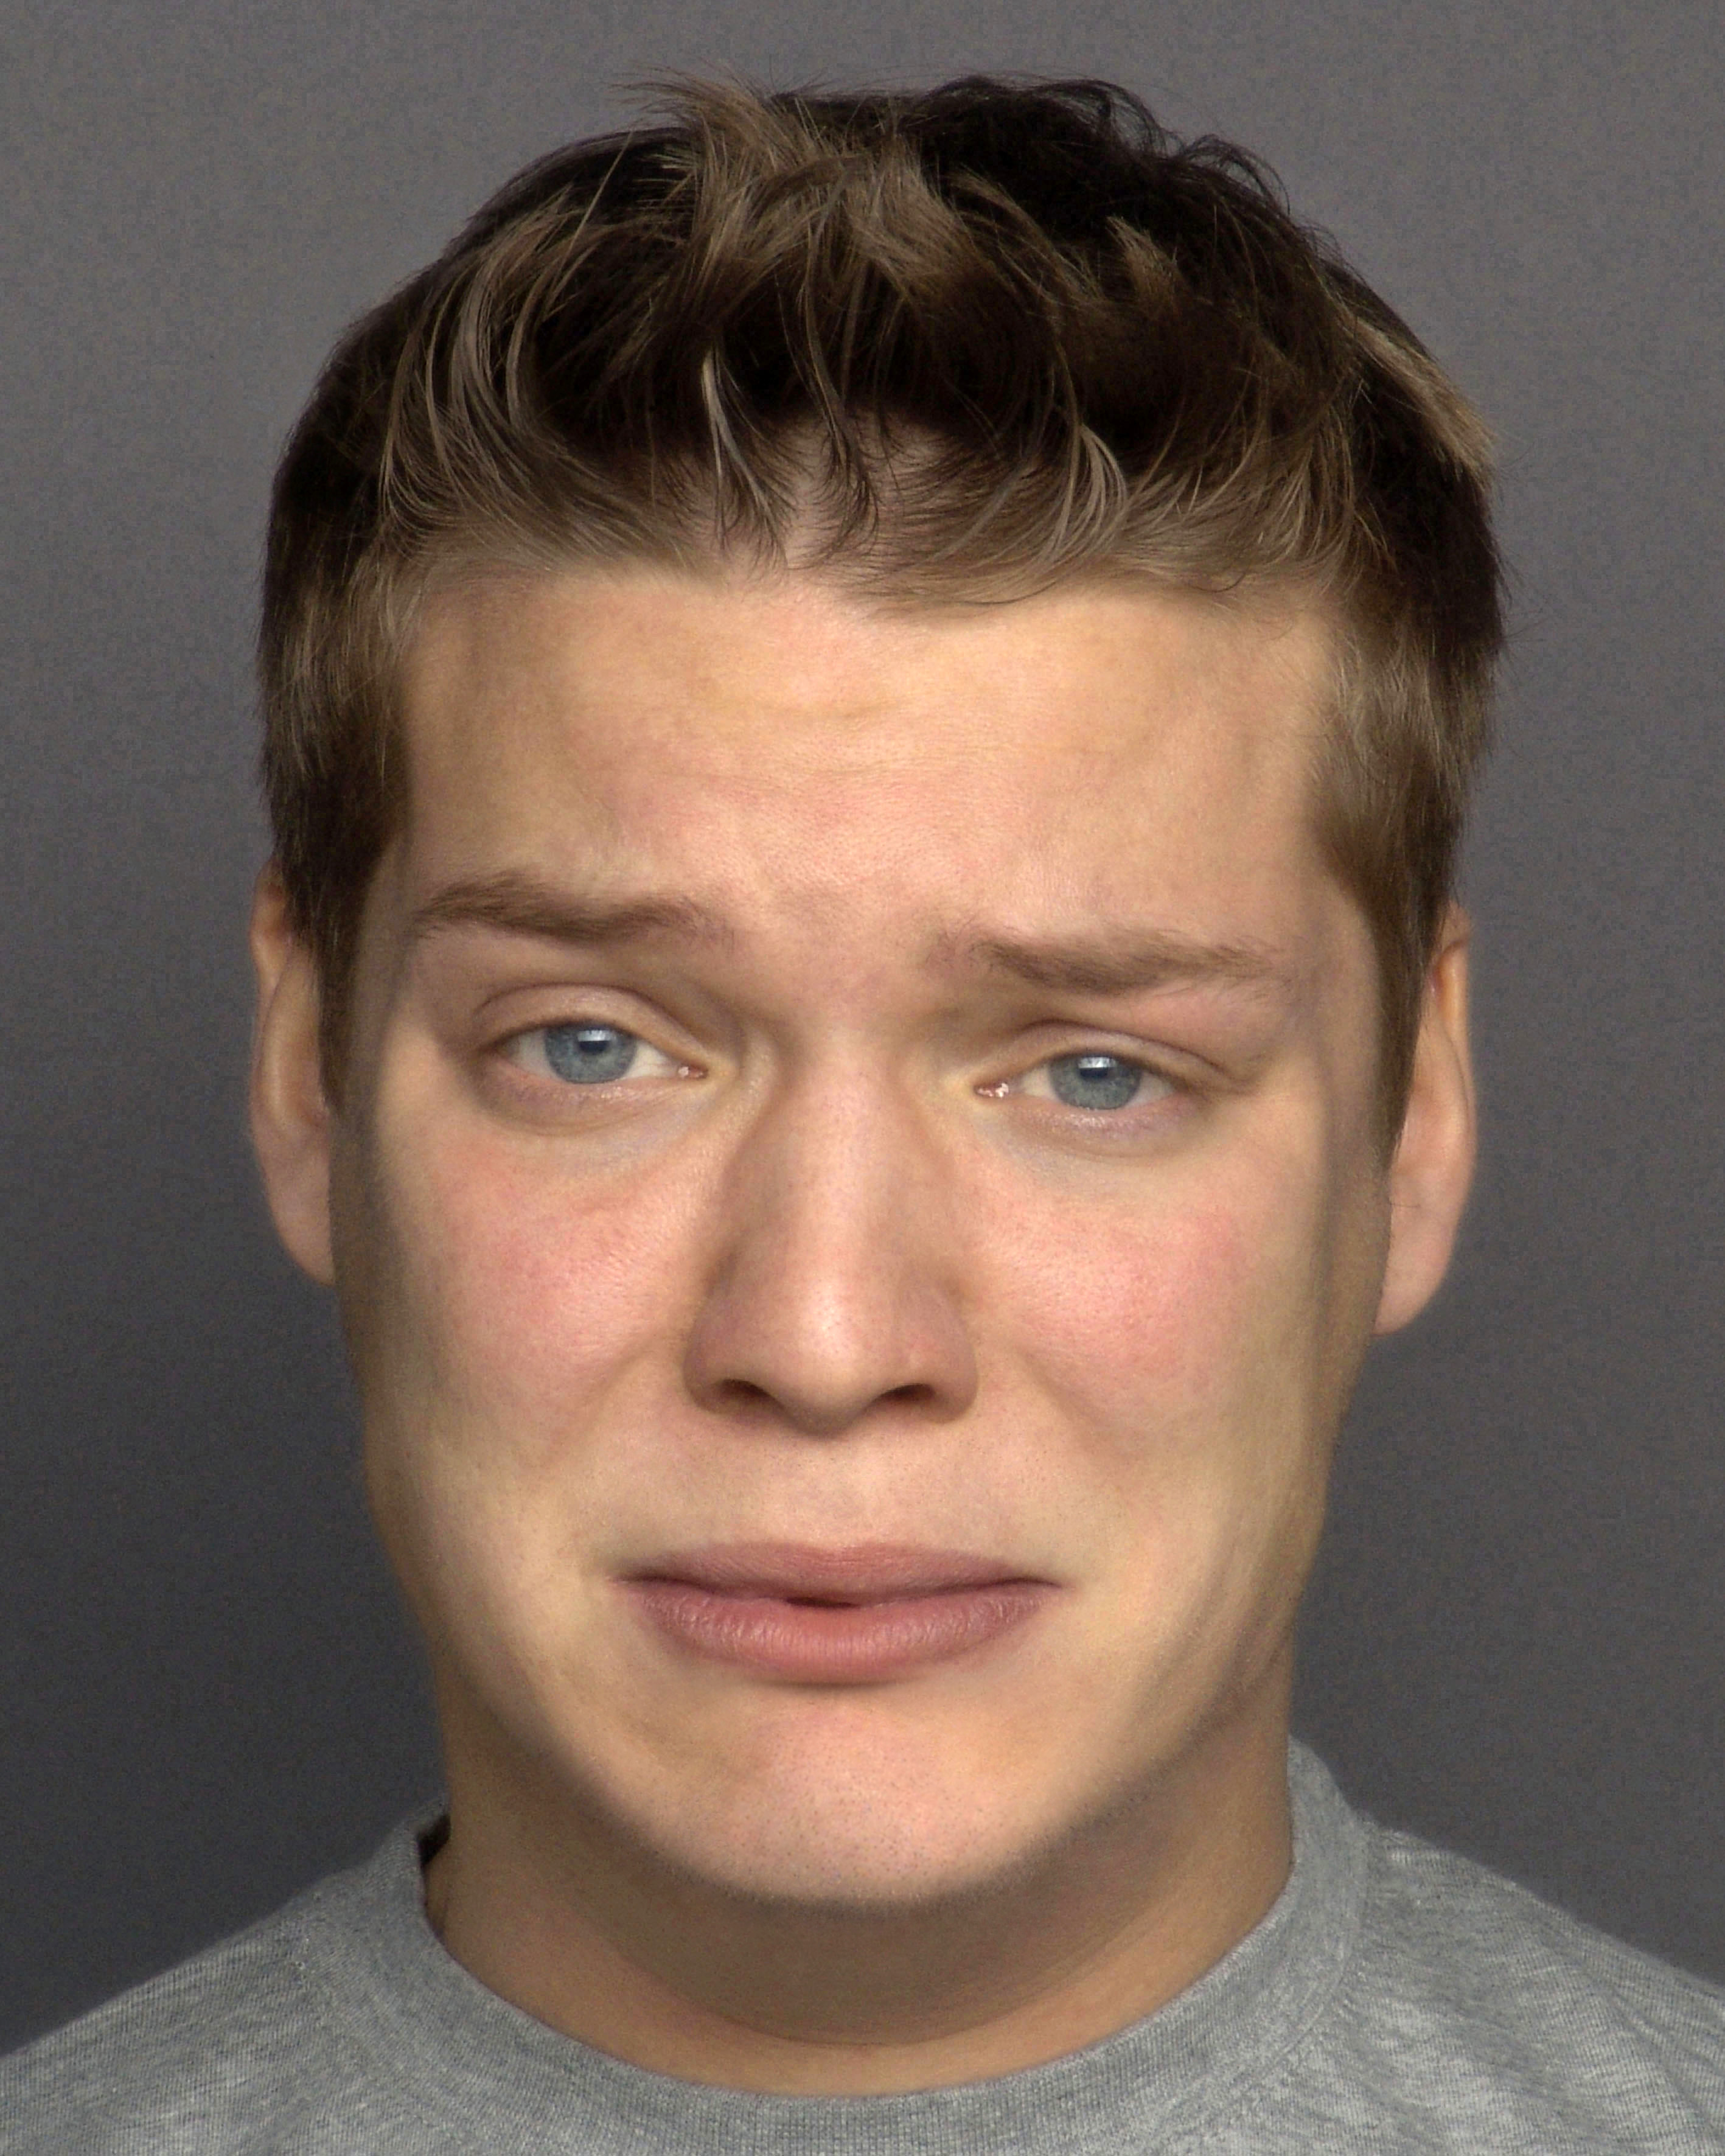
\includegraphics[height=4cm]{zdjęcia/src_img.jpg}
		\subcaption{\label{src_img}}
	\end{subfigure}
	\begin{subfigure}{0.35\textwidth}
		\centering
		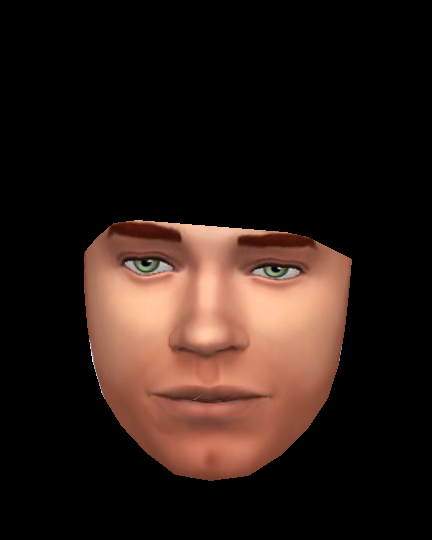
\includegraphics[height=4cm]{zdjęcia/mask_before_avatar.png}
		\subcaption{\label{mask_before_avatar}}
	\end{subfigure}
	\begin{subfigure}{0.35\textwidth}
		\centering
		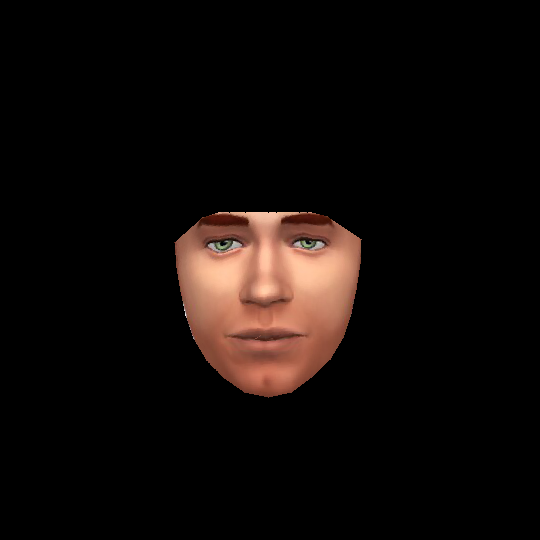
\includegraphics[height=4cm]{zdjęcia/mask_after_avatar.png}
		\subcaption{\label{mask_after_avatar}}
	\end{subfigure}
	\begin{subfigure}{0.35\textwidth}
		\centering
		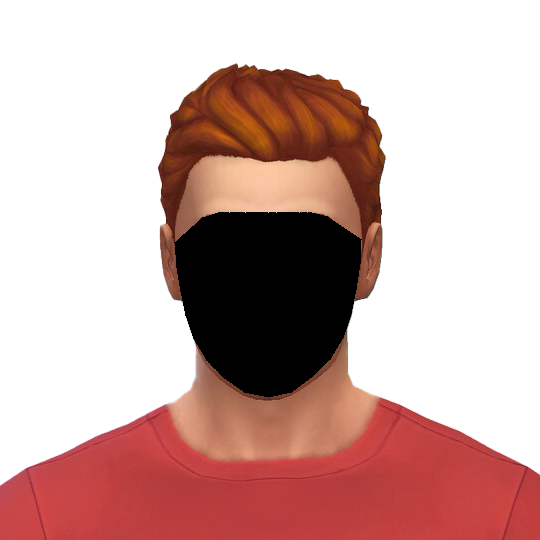
\includegraphics[height=4cm]{zdjęcia/without_face_avatar.png}
		\subcaption{\label{without_face_avatar}}
	\end{subfigure}
	
	\caption{\label{fig:masks}Kolejne kroki działania etapu końcowego}
\end{figure}

Aby podmienienić oblicze awatara na zmodyfikowany obszar wystarczy skorzystać z podstawowej operacji przetwarzania obrazów, czyli funkcji \textit{bitwise\_and()} udostępnionej przez bibliotekę OpenCV. Umożliwia ona zastosowanie na zdjęciu źródłowym maski o wymiarach nowego obszaru twarzy, czego rezultatem jest obraz przedstawiony na Rys. \ref{without_face_avatar}.

\begin{figure}[h]
	\centering
	\begin{subfigure}{0.35\textwidth}
		\centering
		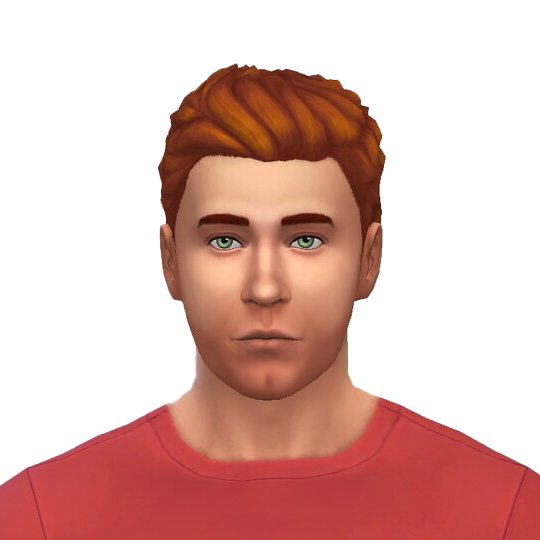
\includegraphics[height=5.5cm]{zdjęcia/avatar.png}
		\subcaption{\label{avatar}}
	\end{subfigure}
	\begin{subfigure}{0.35\textwidth}
		\centering
		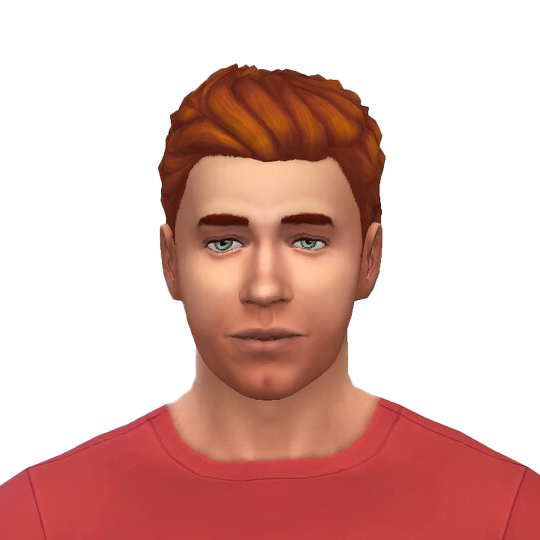
\includegraphics[height=5.5cm]{zdjęcia/result_avatar.png}
		\subcaption{\label{result_avatar}}
	\end{subfigure}
	
	\caption{\label{fig:result}Rezultat działania algorytmu animacji awatara \protect\subref{result_avatar} na zdjęciu źródłowym \ref{fig:masks} \protect\subref{src_img} oraz na przykładowym obrazie awatara \protect\subref{avatar}}
\end{figure}

Po dokonaniu owej operacji wystarczy dodać do siebie obrazy \ref{mask_after_avatar} oraz \ref{without_face_avatar}, aby otrzymać finalny rezultat przedstawiony na Rys. \ref{avatar}, gdzie można obserwować zmodyfikowany wyraz twarzy awatara.

% https://medium.com/featurepreneur/performing-bitwise-operations-on-images-using-opencv-6fd5c3cd72a7
\newpage
% %---------------------------------------------------------------------------

\section{Aplikacja webowa}
Na potrzeby przeprowadzenia ewaluacji algorytmu zaimplementowanego w tej pracy inżynierskiej, stworzono prostą aplikację webową zbudowaną na minimalistycznym szkielecie Flask. Skorzystano również z biblioteki Bootstrap, aby w prosty sposób dostosować wygląd strony do wymagań użytkownika.

Grafika zamieszczona poniżej przedstawia strukturę aplikacji webowej. Umieszczono na niej funkcje, które zostały opisane we wcześniejszych sekcjach oraz pozostałe moduły zaimplementowane na potrzeby stworzenia poprawnie działającej aplikacji.

\begin{figure}[h]
	\centering
	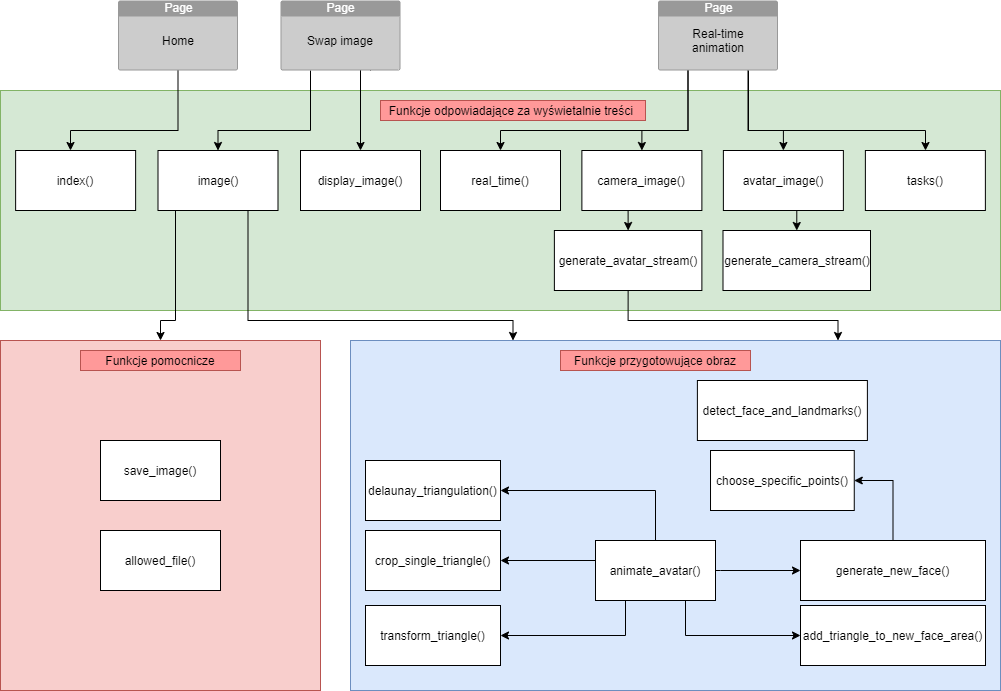
\includegraphics[width=15cm]{zdjęcia/structure_app.png}
	\caption{Struktura aplikacji webowej} 
	\label{fig:structureApp}
\end{figure}

Aplikacja webowa składa się z trzech podstron. Dla dwóch z nich na Rys. \ref{fig:app} przedstawiono wizualizację interfejsów graficznych. Funkcje, które pełnią opisano poniżej.

\begin{enumerate}
    \item Krótka instrukcja zamieszczona na stronie głównej ma na celu zapoznanie użytkownika z możliwościami działania programu.
    \item Zakładka \textit{Select image} umożliwia osobie zainteresowanej wgranie dwóch dowolnych zdjęć, gdzie jedno odpowiada obrazowi źródłowemu, na podstawie którego nastąpi animacja drugiego obrazu. Obsłużono wszelkiego rodzaju błędy, takie jak próba wczytania złego rozszerzenia pliku bądź zdjęcia, na którym nie da się wykryć twarzy i punktów charakterystycznych.
    \item Podstrona \textit{Real-time animation} umożliwia użytkownikowi przetestowanie działania algorytmu w czasie rzeczywistym na wybranym, z czterech możliwych, awatarze. Po przyciśnięciu przycisku \textit{Animate} następuje zastosowanie algorytmu na zdjęciu awatara dla aktualnego obrazu przechwyconego z kamery. W przypadku braku wykrycia twarzy, efekt nie zostanie osiągnięty.
\end{enumerate}

\begin{figure}[h]
	\centering
	\subfloat[Wybór dwóch zdjęć wykorzystanych do animacji]{
	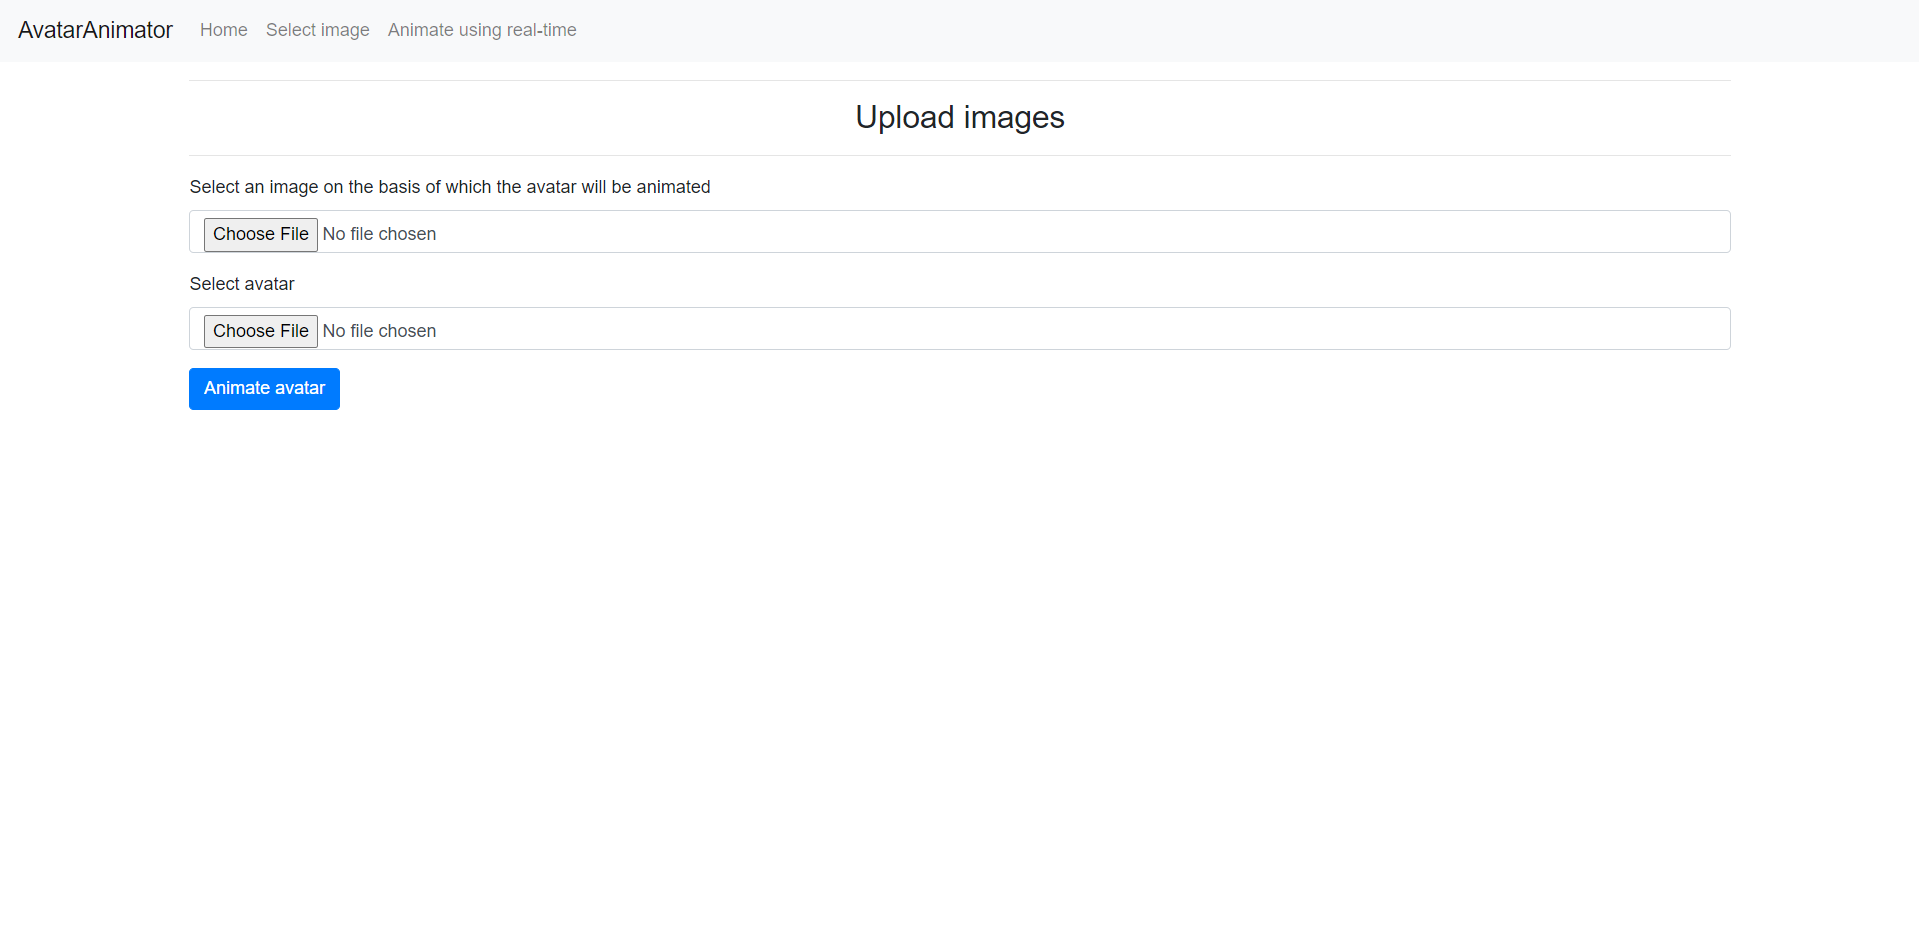
\includegraphics[height=8cm]{zdjęcia/select_images.PNG}
	}\quad
	\subfloat[Wykorzystanie do animacji obrazu z kamery]{
	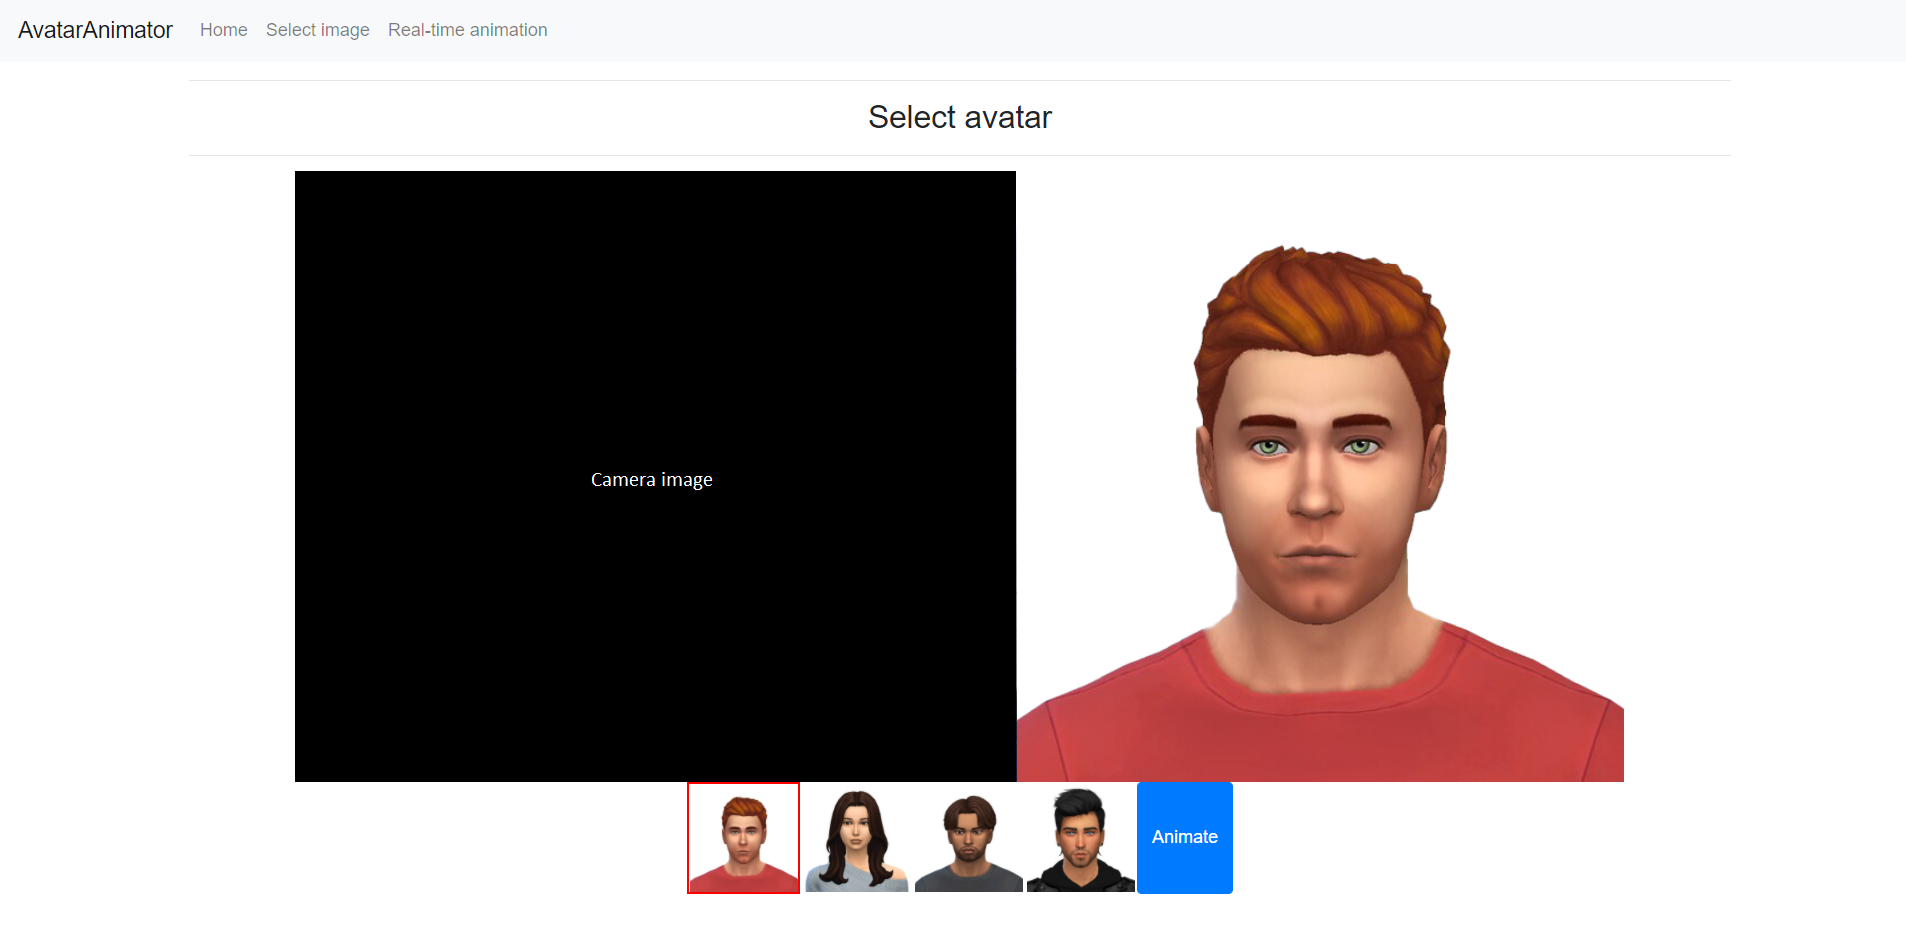
\includegraphics[height=8cm]{zdjęcia/animate_real_time.PNG}
	}
	\caption{\label{fig:app}Interfejsy graficzne aplikacji webowej}
\end{figure}


